\documentclass[12pt, a4paper]{article}
\usepackage{fontspec}
\setmainfont{Times New Roman}
\usepackage[UTF8]{ctex}
\usepackage{listings}
\usepackage{array}
\usepackage{geometry}
\geometry{a4paper, scale=0.75}
\usepackage{ctex}
\usepackage{amsmath}
\usepackage{epsfig}
\usepackage{graphicx}
\usepackage{epstopdf}
\usepackage{cite}
\usepackage{indentfirst}
\setlength{\parindent}{2em}
\setlength\parskip{.3 \baselineskip}
\usepackage{graphicx}
\usepackage{float}
\usepackage{subfigure}

\begin{document}
	\begin{center}
		\vspace{0.2in}
		\noindent{\fontsize{20pt}{1em}\selectfont\textbf{通信电路\quad 第二周作业}} \\ [12pt]
		\noindent{\fontsize{20pt}{1em}\textbf{Cadence报告}}  \\ [12pt]
		{\fontsize{14pt}{1.2em}\selectfont
			刘开济\\ [10pt]
			2019010973 \\ [10pt]
		}
	\end{center}
    \section{用传输线实现电容电感}
    \subsection{感抗L型网络实现低通/高通最大功率传输匹配}
    由纸质作业不难得到基于电容、电感的电路设计:
    \begin{figure}[htbp]
    	\centering
    	\begin{minipage}[t]{0.48\textwidth}
    		\centering
    		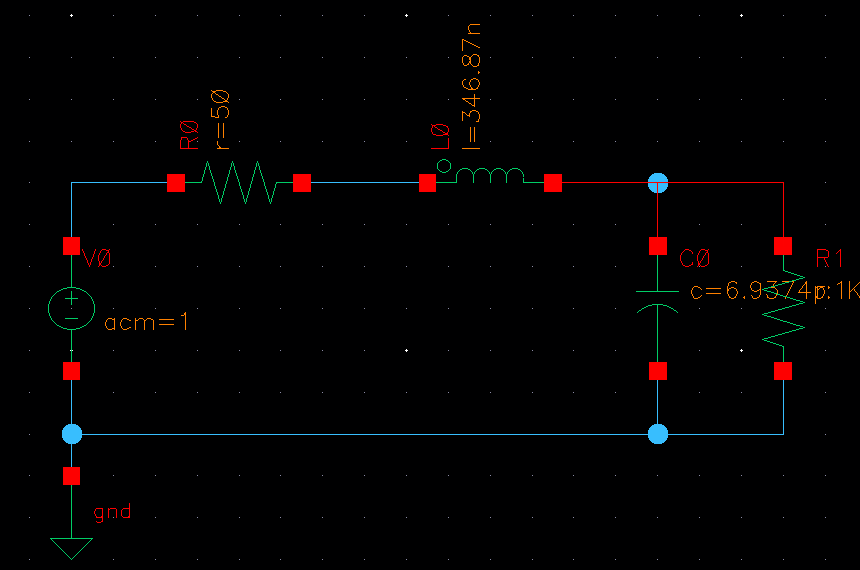
\includegraphics[width=6cm]{L-LP-STD-circuit}
    		\caption{L型低通匹配电路}
    		\label{fig1.1}
    	\end{minipage}
    	\begin{minipage}[t]{0.48\textwidth}
    		\centering
    		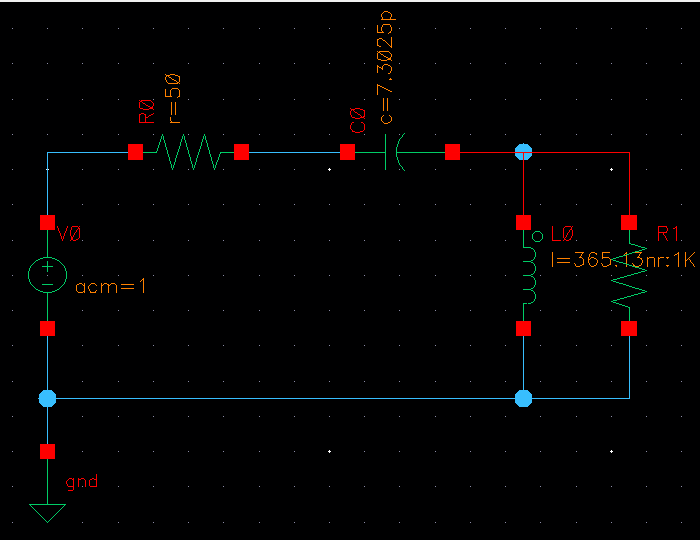
\includegraphics[width=6cm]{L-HP-STD-circuit}
    		\caption{L型高通匹配电路}
    	\end{minipage}
    \end{figure}\par
    其中有关键参数:
    $$
    \begin{cases}
    	L_{LPF} = 346.87nH \\
    	C_{LPF} = 6.9374pF \\
    	L_{HPF} = 365.13nH\\
    	C_{HPF} = 7.3025pF 
    \end{cases}
    $$\par
    考察其幅频特性。\par
    分别考虑其在$50MHz-200MHz$与$50MHz-500MHz$的幅频特性,可知其在很宽的频带内比较平坦。
     \begin{figure}[htbp]
    	\centering
    	\begin{minipage}[t]{0.48\textwidth}
    		\centering
    		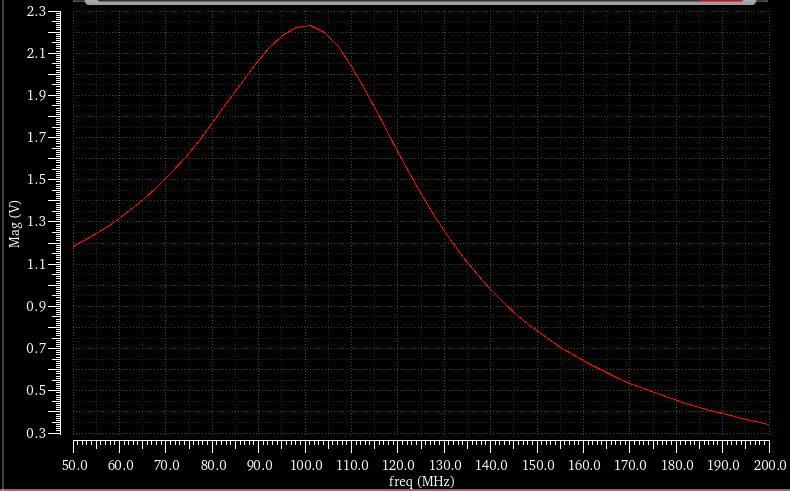
\includegraphics[width=6cm]{L-LP-STD-plot-50-200}
    		\caption{LPF\ 50MHz-200MHz范围幅频特性}
    	\end{minipage}
    	\begin{minipage}[t]{0.48\textwidth}
    		\centering
    		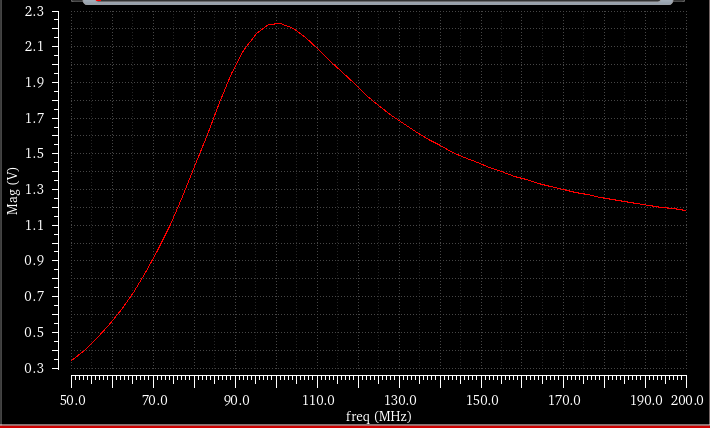
\includegraphics[width=6cm]{L-HP-STD-plot-50-200}
    		\caption{HPF\ 50MHz-200MHz范围幅频特性}
    	\end{minipage}
    \end{figure}\par
    \begin{figure}[htbp]
    	\centering
    	\begin{minipage}[t]{0.48\textwidth}
    		\centering
    		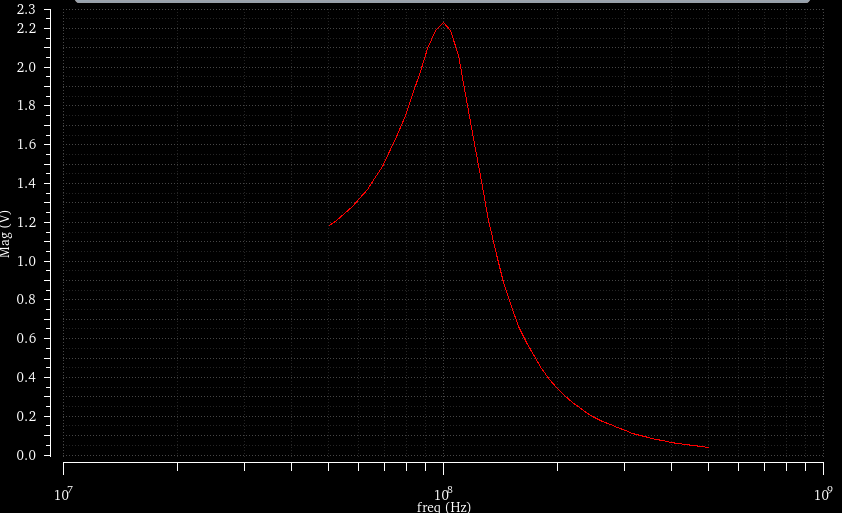
\includegraphics[width=6cm]{L-LP-STD-plot-50-500}
    		\caption{LPF\ 50MHz-500MHz范围幅频特性}
    	\end{minipage}
    	\begin{minipage}[t]{0.48\textwidth}
    		\centering
    		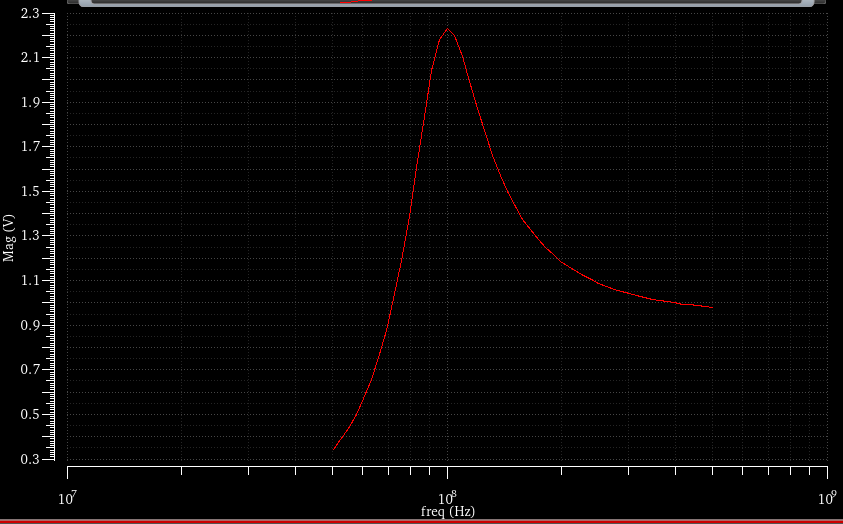
\includegraphics[width=6cm]{L-HP-STD-plot-50-500}
    		\caption{HPF\ 50MHz-500MHz范围幅频特性}
    	\end{minipage}
    \end{figure}\par
    \subsection{传输线L型网络实现低通/高通最大功率传输匹配}
    我们先考察传输线等效电感电容的理论。\par
    对于理想传输线,输入阻抗满足:
    \begin{equation}
    	Z_{in} = Z_0 \frac{Z_L + j Z_0 tan \beta l}{Z_0 + j Z_L tan \beta l}
    \end{equation}\par
    若取终端短路,对$\frac{1}{8}$波长传输线就有:
    \begin{equation}
    	Z_{in}|_{short, \frac{1}{8}\lambda} = jZ_0 
    \end{equation}\par
    可知$frac{1}{8}$波长终端短路传输线可以等效为电感。若取终端开路,则相应有:
    \begin{equation}
    	Z_{in}|_{open, \frac{1}{8}\lambda} = \frac{Z_0}{j} 
    \end{equation}\par
    可知$\frac{1}{8}$波长终端开路传输线可以等效为电容。考虑匹配频点$f_0 = 100MHz$,根据之前感抗LC匹配网络,可以解得对应传输线的特征阻抗,其参数为:
    $$
    \begin{cases}
    	Z_0|{LPF, L} = 217.9449 \Omega \\
    	Z_0|{LPF, C} = 229.4157 \Omega \\
    	Z_0|{HPF, C} = 217.9449 \Omega \\
    	Z_0| {HPF, L} = 229.4157 \Omega
    \end{cases}
    $$
    仿真电路如下:
     \begin{figure}[H]
    	\centering
    	\subfigure[传输线LPF\ schematic]{
    		\begin{minipage}[t]{0.48\linewidth}
    			\centering
    			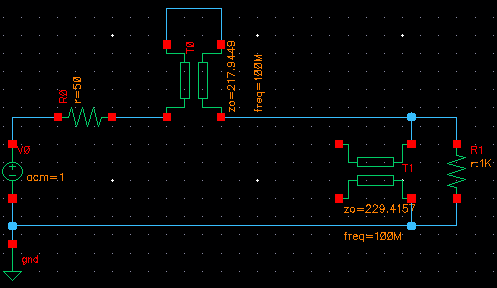
\includegraphics[width=6cm]{L-LP-TLINE-circuit}
    			% \caption{传输线LPF\ 50MHz-200MHz幅频特性}
    			%\caption{fig1}
    		\end{minipage}%
    	}%
    	\subfigure[传输线HPF\  schematic]{
    		\begin{minipage}[t]{0.48\linewidth}
    			\centering
    			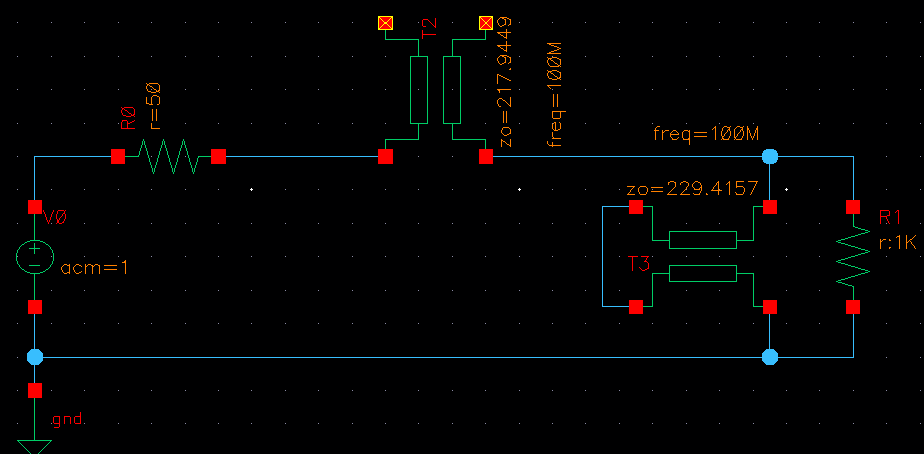
\includegraphics[width=6cm]{L-HP-TLINE-circuit}
    			% \caption{传输线LPF\ 50MHz-500MHz幅频特性}
    			%\caption{fig2}
    		\end{minipage}%
    	}%
    	%这个回车键很重要 \quad也可以 
    	
    	\centering
    	\caption{传输线L型匹配电路设计}
    \end{figure}
   \begin{figure}[H]
   	\centering
   	\subfigure[传输线LPF\ 50MHz-200MHz幅频特性]{
   		\begin{minipage}[t]{0.48\linewidth}
   			\centering
   			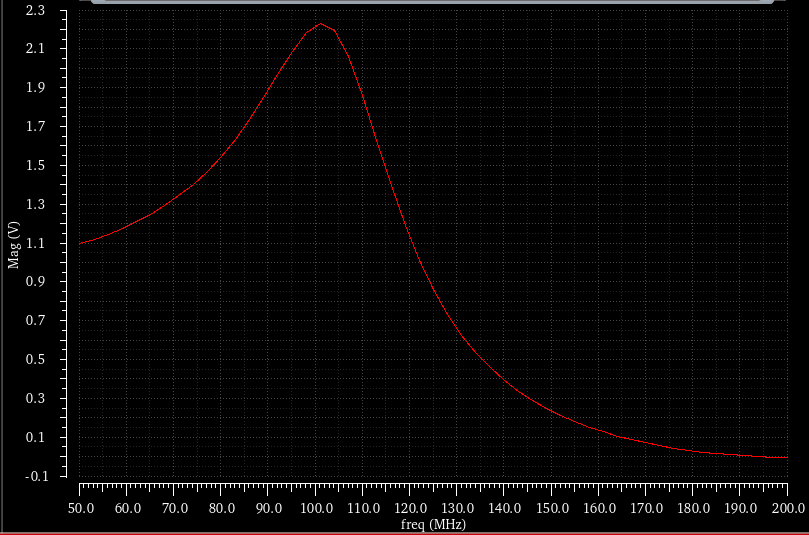
\includegraphics[width=6cm]{L-LP-TLINE-plot-50-200}
   			% \caption{传输线LPF\ 50MHz-200MHz幅频特性}
   			%\caption{fig1}
   		\end{minipage}%
   	}%
   	\subfigure[传输线LPF\ 50MHz-500MHz幅频特性]{
   		\begin{minipage}[t]{0.48\linewidth}
   			\centering
   			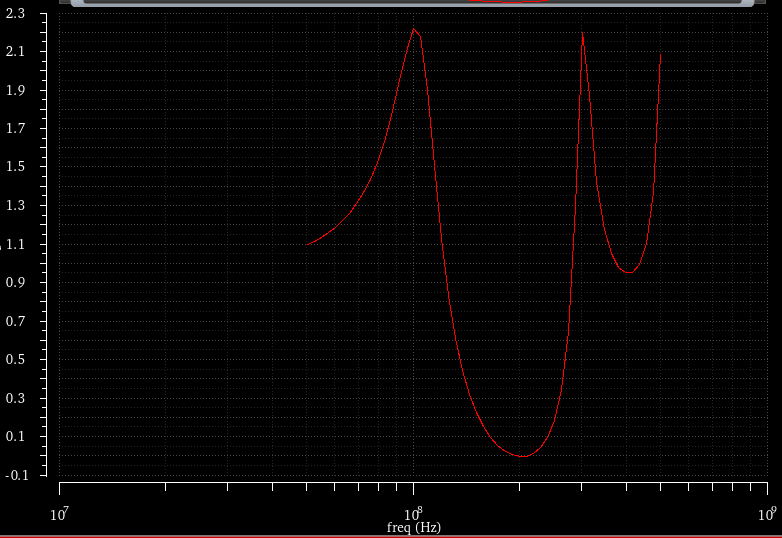
\includegraphics[width=6cm]{L-LP-TLINE-plot-50-500}
   			% \caption{传输线LPF\ 50MHz-500MHz幅频特性}
   			%\caption{fig2}
   		\end{minipage}%
   	}%
   	%这个回车键很重要 \quad也可以 
   	\par
   	\subfigure[传输线HPF\ 50MHz-200MHz幅频特性]{
   		\begin{minipage}[t]{0.48\linewidth}
   			\centering
   			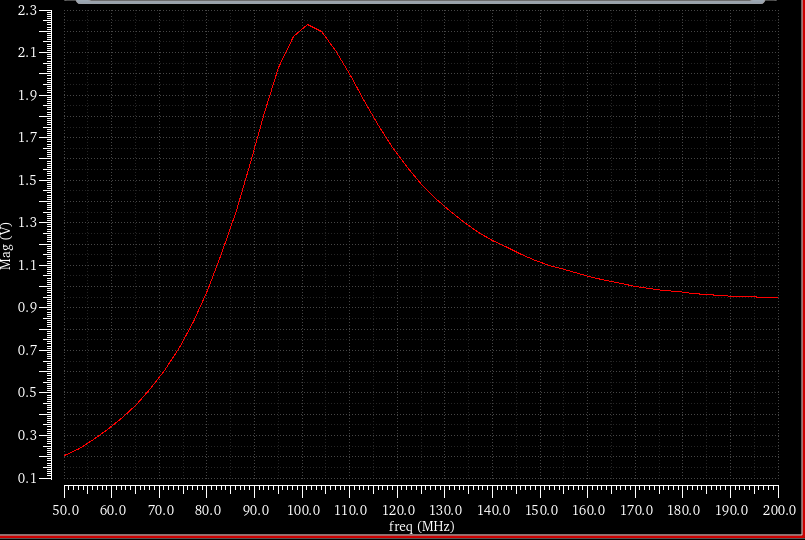
\includegraphics[width=6cm]{L-HP-TLINE-plot-50-200}
   			% \caption{传输线HPF\ 50MHz-200MHz幅频特性}
   			%\caption{fig2}
   		\end{minipage}
   	}%
   	\subfigure[传输线HPF\ 50MHz-1GHz幅频特性]{
   		\begin{minipage}[t]{0.48\linewidth}
   			\centering
   			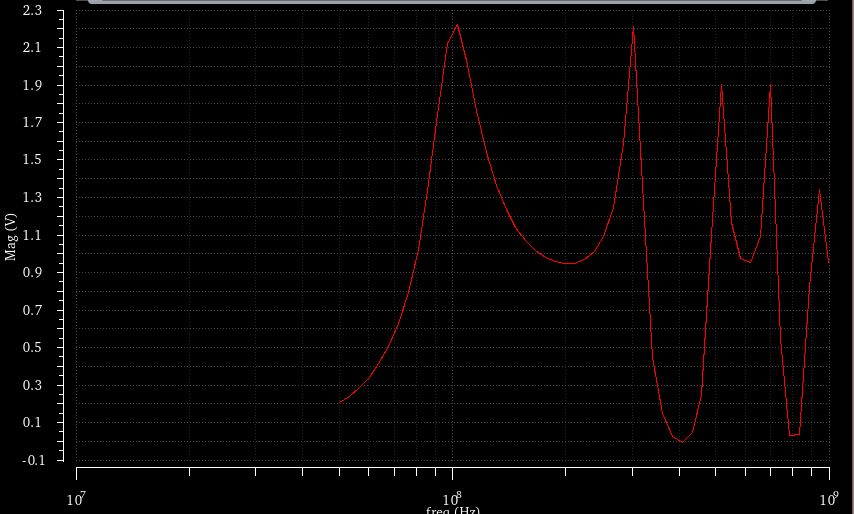
\includegraphics[width=6cm]{L-HP-TLINE-plot-50-1000}
   			% \caption{传输线HPF\ 50MHz-1GHz幅频特性}
   			%\caption{fig2}
   		\end{minipage}
   	}%
   	
   	\centering
   	\caption{传输线L型匹配网络幅频特性}
   \end{figure}\par
   我们发现,在匹配频点附近,传输线电路的幅频特性与LC感抗电路相近。但在高频段,传输线电路出现了明显的选频尖峰。\par
   \section{用Butterworth方法实现低通/带通滤波器}
   \subsection{Butterworth低通滤波}
   理论分析按照课件操作依样画葫芦。本滤波器实现比较简单,是一个二阶Butterworth LPF。
   \begin{figure}[H]
   	    \centering
   	    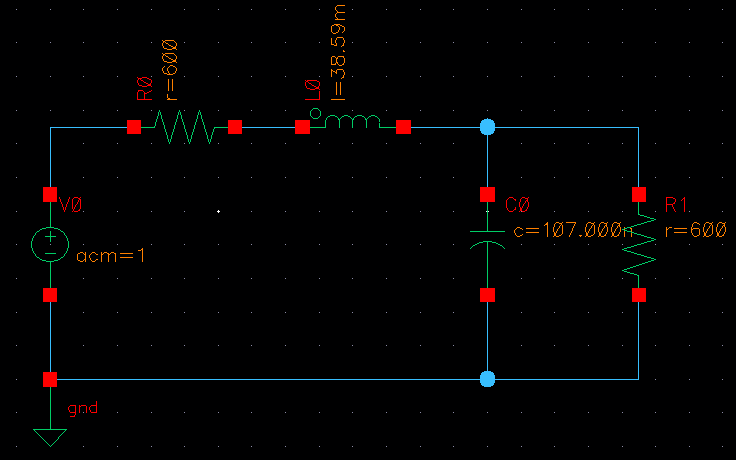
\includegraphics[width = 0.8\textwidth]{ButterworthLPF-circuit}
   	    \caption{LPF电路}
   	    \label{Fig2.1}
   \end{figure}
    考察其幅频特性,有:
    \begin{figure}[H]
    	\centering
    	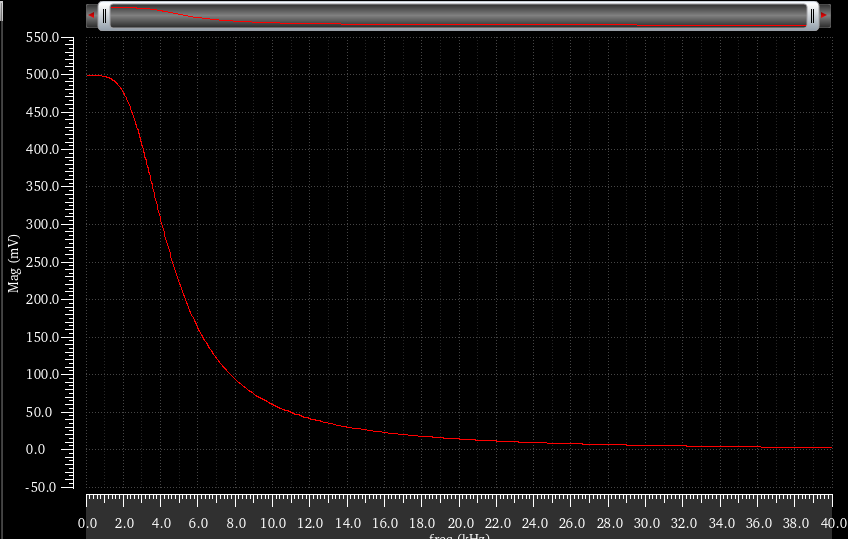
\includegraphics[width = 0.8\textwidth]{ButterworthLPF-plot}
    	\caption{LPF幅频特性}
    \end{figure}\par
   
   检验设计参数,其中有额定电压$V_0 = 500mV$有:\par
   \begin{center}
   	\tabcolsep8pt
   	\arrayrulewidth2pt
   	\begin{tabular}{| c | c | c | }
   		\hline
   		采样频率$f$ &  采样压降$V_{smpl}$ & 衰减系数$\alpha_s = 20 || log_{10}(\frac{V_{smpl}}{V_0}) ||$  \\
   		\hline
   		2.01502 kHz & 474.6816mV & 0.4514 \\
   		\hline
   		29.7305 kHz & 6.939613mV & 37.1527 \\
   		\hline
   	\end{tabular}
   \end{center} \par
    可见该设计符合需求。
    \subsection{Butterworth带通滤波}
    理论分析仍参考课件,本滤波器低通原型至少为一个三阶Butterworth滤波器。\par
    \begin{figure}[H]
    	\centering
    	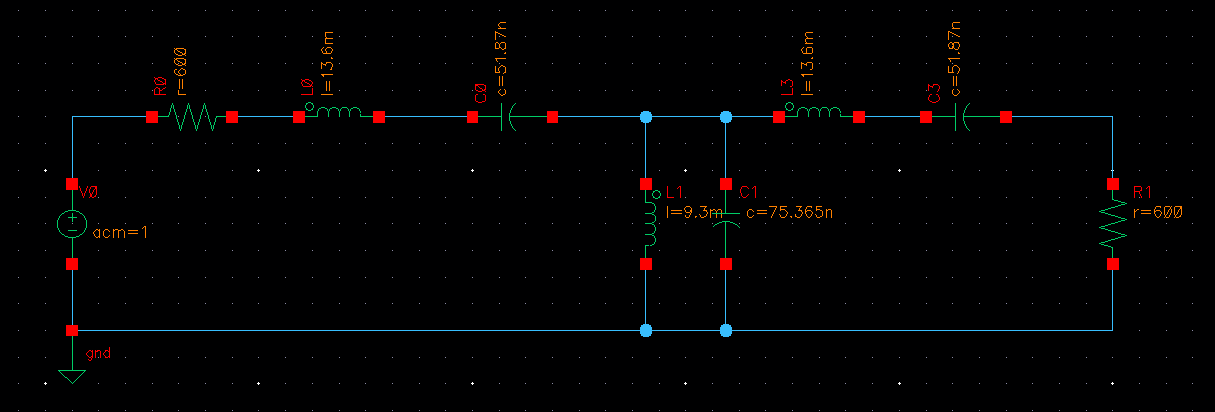
\includegraphics[width = 0.8\textwidth]{ButterworthBPF-circuit}
    	\caption{BPF电路}
    \end{figure}
    考察其幅频特性,有:
    \begin{figure}[H]
    	\centering
    	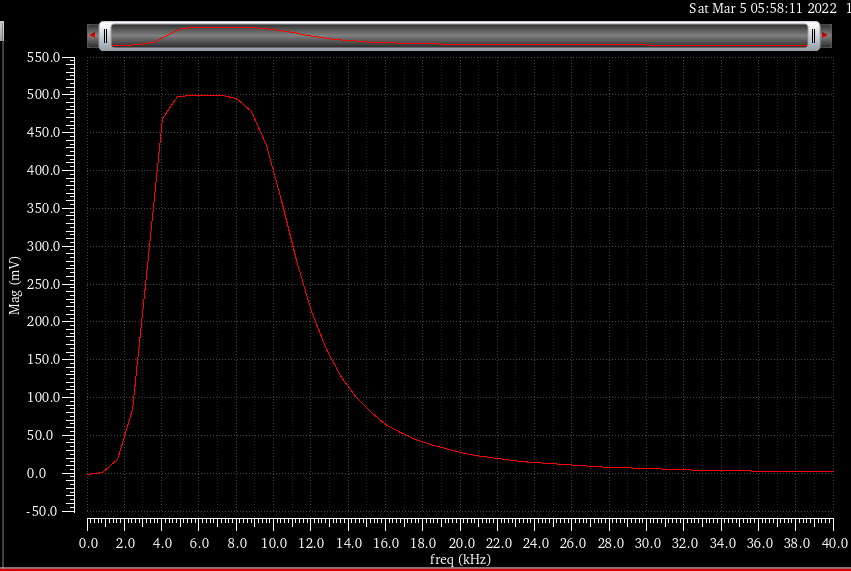
\includegraphics[width = 0.8\textwidth]{ButterworthBPF-plot}
    	\caption{BPF幅频特性}
    \end{figure}\par
    分别考察其通带与阻带衰减系数。
    \begin{center}
    	\tabcolsep8pt
    	\arrayrulewidth2pt
    	\begin{tabular}{| c | c | c | }
    		\hline
    		采样频率$f$ &  采样压降$V_{smpl}$ & 衰减系数$\alpha_s = 20 || log_{10}(\frac{V_{smpl}}{V_0}) ||$  \\
    		\hline
    		3.70488 kHz & 398.2865mV & 1.9755 \\
    		\hline
    		9.70885 kHz & 424.1371mV & 1.4293 \\
    		\hline
    		29.6kHz & 7.588475mV & 36.3763 \\
    		\hline
    	\end{tabular}
    \end{center} \par
     通带和阻带衰减系数满足设计要求。实验用Matlab代码打包上传。
\end{document}